%%%%%%%%%%%%%%%%%%%%%%%%%%%%%%%%%%%%%%%%%%%%%%%%%%%%%%%%%%%%%%%
%
% Welcome to Overleaf --- just edit your LaTeX on the left,
% and we'll compile it for you on the right. If you open the
% 'Share' menu, you can invite other users to edit at the same
% time. See www.overleaf.com/learn for more info. Enjoy!
%
%%%%%%%%%%%%%%%%%%%%%%%%%%%%%%%%%%%%%%%%%%%%%%%%%%%%%%%%%%%%%%%
\documentclass{beamer}
 \usetheme[options]{Boadilla}
 % paquets pour le français
 \usepackage{tikz}
 \usepackage{multicol}
 \usepackage[T1]{fontenc}
 \usepackage[utf8]{inputenc}
\usepackage{minted}
\definecolor{LightGray}{gray}{0.9}
  \title{Programmation C: Pointeur}
  \author{ \textsc{Ibrahim ALAME}}\institute{ESIEE}
\date{13/10/2023}
\begin{document}
\maketitle
 \begin{frame}[fragile]
  \frametitle{Pointeurs}
  \begin{block}{Définition: L'opérateur \&}
 L'opérateur adresse \& retourne l'adresse d'une variable en mémoire en hexadécimal (4 octets).
\end{block}

\begin{minted}[
%frame=lines,
framesep=2mm,
baselinestretch=1.2,
bgcolor=LightGray,
fontsize=\footnotesize,
% linenos
]{c}
#include <stdio.h>
int main(){ 
    int i = 5;
	printf(" Valeur de i: %d \n",i);
	printf(" Valeur de son adresse : %p \n",&i);
    return 0; 
}
\end{minted}
{\tiny
\begin{verbatim}
 Valeur de i: 5 
 Valeur de son adresse : 0x7ffcc91b9784 

...Program finished with exit code 0
Press ENTER to exit console.
\end{verbatim}
}
\begin{itemize}
\item L'adresses d'une variable correspond à l'adresse de début de la variable dans la mémoire.
\end{itemize}


\end{frame}
  
  %%%%%%%%%%%%%%%%%%%%%%%%%%%%%%%%%%%%%%%%%%%%%%%%%%%%%%%%%%%%%%%%%

\begin{frame}[fragile]
\frametitle{Pointeur}
\begin{block}{Qu'est-ce qu'un pointeur?}
C'est une variable qui contient l'adresse d'une autre variable. On dit que le pointeur pointe sur la variable.
\end{block}
\begin{multicols}{2}
\begin{minted}[
%frame=lines,
framesep=2mm,
baselinestretch=1.2,
bgcolor=LightGray,
fontsize=\footnotesize,
% linenos
]{c}  
#include <stdio.h>
int main(){ 
    int *p, X;
    X=5;
    p=&X;
    printf("X= %d \n",X);
    printf("Son adresse: p=%p",p);
    return 0; 
}
\end{minted}
{\tiny
\begin{verbatim}
X= 5 
Son adresse: p=0x7fffa85ecddc

...Program finished with exit code 0
Press ENTER to exit console.
\end{verbatim}
}
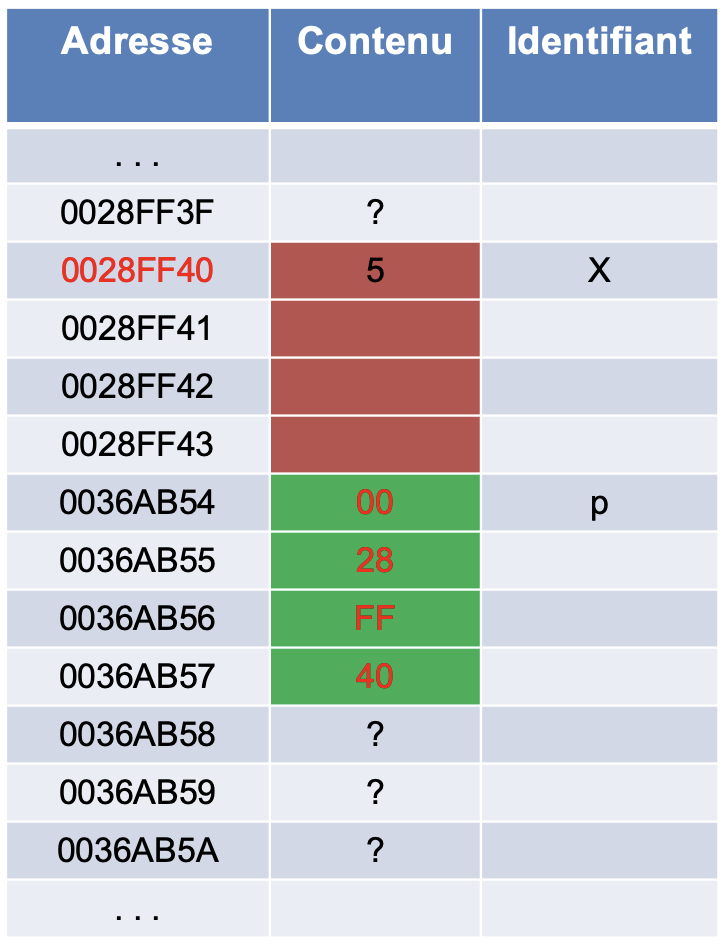
\includegraphics[scale=0.4]{pointeur1.png} 
\end{multicols}
\end{frame}
  %%%%%%%%%%%%%%%%%%%%%%%%%%%%%%%%%%%%%%%%%%%%%%%%%%%%%%%%%%%%%%%%%
  
  
\begin{frame}[fragile]
\frametitle{Les pointeurs}

\begin{block}{Qu'est-ce qu'un pointeur?}
\begin{itemize}
\item Une variable de type pointeur se déclare à l'aide de l'objet pointé précédé du symbole * (opérateur d'indirection).
\item L'opérateur  *  désigne le contenu de l'adresse,
\end{itemize}
\end{block}

\begin{itemize}
\item Exemple :
\begin{minted}[
%frame=lines,
framesep=2mm,
baselinestretch=1.2,
bgcolor=LightGray,
fontsize=\footnotesize,
% linenos
]{c}
int *pi;   	// pi est un pointeur pointant sur un entier  
char *pc;	// pc est un pointeur pointant sur un char
float *pf;	// pf est un pointeur pointant sur un float
\end{minted}
\item Exemple :
\begin{minted}[
%frame=lines,
framesep=2mm,
baselinestretch=1.2,
bgcolor=LightGray,
fontsize=\footnotesize,
% linenos
]{c}
int *pi, X; // pi est un pointeur pointant sur un entier
pi = &X;	 // on initialise le pointeur pi  
*pi = 5;    // On charge l'entier pointé par pi avec la 				
             // valeur 5, c'est en fait X
\end{minted}
\end{itemize}

\end{frame}
  


 
%%%%%%%%%%%%%%%%%%%%%%%%%%%%%%%%%%%%%%%%%%%%%%%%%%%%%%%%%%%%%%%
\begin{frame}[fragile]
\frametitle{Pointeurs: L'arithmétique des pointeurs.}

\begin{multicols}{2}
On déplace  un pointeur dans la mémoire à l'aide des opérateurs d'addition, de soustraction, d'incrémentation, de décrémentation.

On ne peut le déplacer que d'un nombre de cases mémoire multiple de la taille de la variable en mémoire.
\begin{minted}[
%frame=lines,
framesep=2mm,
baselinestretch=1.2,
bgcolor=LightGray,
fontsize=\footnotesize,
% linenos
]{c}  
    int *pi;   	
    char *pc;	
    *pi = 5;	
    *pc = 'A';
\end{minted}

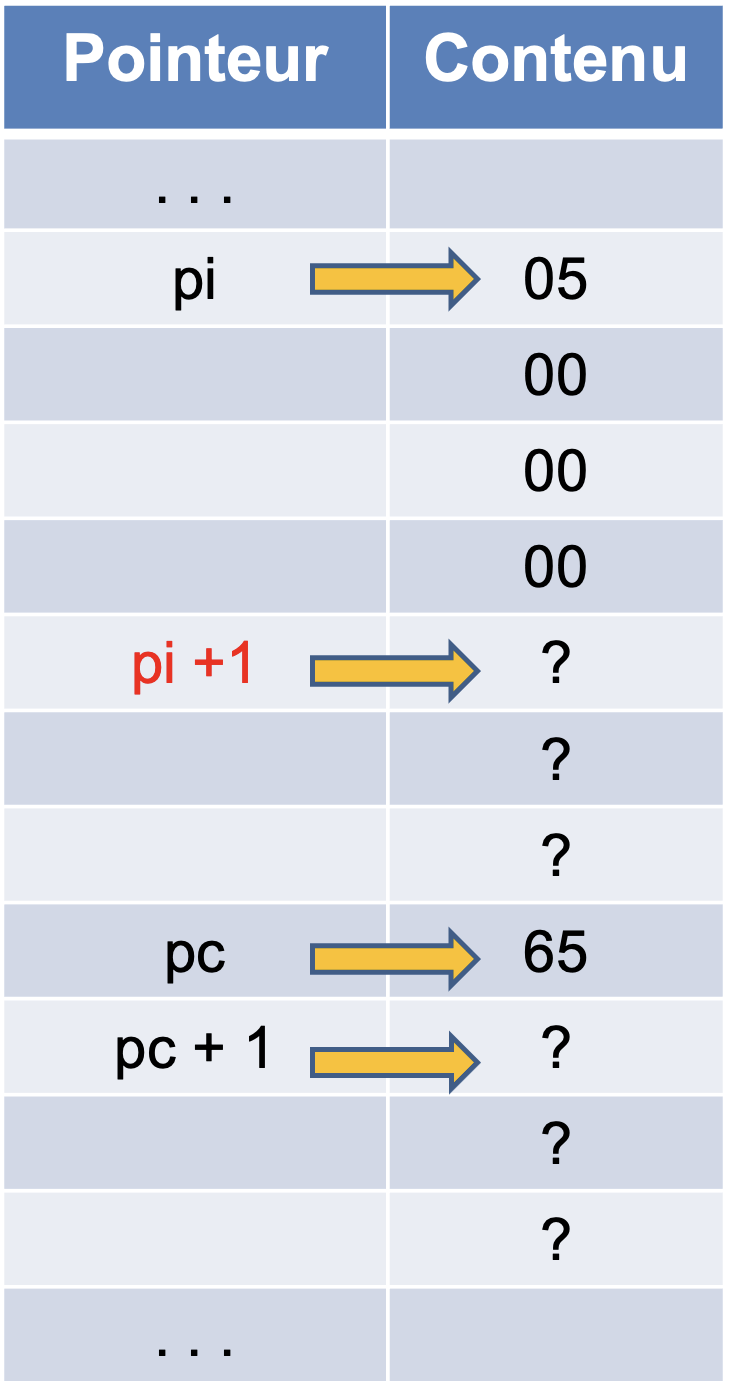
\includegraphics[scale=0.3]{pointeur2.png} 
\end{multicols}

\end{frame}
  
  
 
%%%%%%%%%%%%%%%%%%%%%%%%%%%%%%%%%%%%%%%%%%%%%%%%%%%%%%%%%%%%%%%

\begin{frame}[fragile]
\frametitle{Pointeurs: L'arithmétique des pointeurs.}
\begin{minted}[
%frame=lines,
framesep=2mm,
baselinestretch=1.2,
bgcolor=LightGray,
fontsize=\footnotesize,
% linenos
]{c}
int *pi; // pi pointe sur un objet de type entier	(4 octets)
char *pc; // pc pointe sur un objet de type char (1 octet)
float *pf; // pf pointe sur un objet de type float (4 octets)
*pi = 145; // 145 est le contenu de la case mémoire pi
*(pi+1) = 200; // 200 est de contenu des cases mémoires 4 cases  après pi
*(pi+2)= 500; // 500 est le contenu des cases mémoires 8 cases après pi
*pc = 'A'; // la case mémoire pc contient le code ASCII de A = 65
pc--;	 // on décrémente la valeur du pointeur pc de 1
*pf = 1.5; // 1,5 est stocké dans la case mémoire pf et les 4  suivantes
pf++; // on incrémente la valeur du pointeur pf de 4 cases mémoires
         // qui correspond à la taille d'un float
\end{minted}
\end{frame}
%%%%%%%%%%%%%%%%%%%%%%%%%%%%%%%%%%%%%%%%%%%%%%%%%%%%%%%%%%%%%%%%%

\begin{frame}[fragile]
\frametitle{Pointeurs: L'arithmétique des pointeurs.}
\begin{minted}[
%frame=lines,
framesep=2mm,
baselinestretch=1.2,
bgcolor=LightGray,
fontsize=\footnotesize,
% linenos
]{c}
int *pi,*qi, i;   	
pi = qi; // autorisé 
i = pi + qi; // interdit : on ne peut pas additionner deux pointeurs
                 // ça n'a pas de sens
i = pi-qi; // autorisé: donne le nombre d'objets entre les deux pointeurs
I = pi*qi; // interdit: on ne peut pas multiplier deux pointeurs
              // ça n'a pas de sens
\end{minted}
\end{frame}

%%%%%%%%%%%%%%%%%%%%%%%%%%%%%%%%%%%%%%%%%%%%%%%%%%%%%%%%%%%%%%%%%

\begin{frame}[fragile]
\frametitle{Pointeur : passage par valeur}

Exemple : Fonction permuter

\begin{minted}[
%frame=lines,
framesep=2mm,
baselinestretch=1.2,
bgcolor=LightGray,
fontsize=\footnotesize,
% linenos
]{c}
#include <stdio.h>
void permute (int a, int b) {
    int tmp;
    tmp=a;
    a=b;
    b=tmp;
}
int main () {
    int x=10, y =20;
    printf("avant : x=%d, y=%d \n", x,y);
    permute (x,y);
    printf("apres: x=%d, y=%d \n", x,y);
    return 0;
}
\end{minted}
{\tiny
\begin{verbatim}
avant: x=10, y=20
après: x=10, y=20
\end{verbatim}
}
\end{frame}

%%%%%%%%%%%%%%%%%%%%%%%%%%%%%%%%%%%%%%%%%%%%%%%%%%%%%%%%%%%%%%%%%

\begin{frame}[fragile]
\frametitle{Pointeur : passage par référence}

Exemple : Fonction permuter

\begin{minted}[
%frame=lines,
framesep=2mm,
baselinestretch=1.2,
bgcolor=LightGray,
fontsize=\footnotesize,
% linenos
]{c}
#include <stdio.h>
void permute (int* a, int* b) {
    int tmp;
    tmp= *a;
    *a = *b;
    *b = tmp;
}
int main () {
    int x=10, y =20;
    printf("avant : x=%d, y=%d \n", x,y);
    permute (&x,&y);
    printf("apres: x=%d, y=%d \n", x,y);
    return 0;
}
\end{minted}
{\tiny
\begin{verbatim}
avant: x=10, y=20
après: x=20, y=10
\end{verbatim}
}
\end{frame}

%%%%%%%%%%%%%%%%%%%%%%%%%%%%%%%%%%%%%%%%%%%%%%%%%%%%%%%%%%%%%%%%%


\begin{frame}[fragile]
\frametitle{Pointeurs et tableaux}
En C, il existe une relation très étroite entre tableaux et pointeurs. Ainsi, chaque opération avec des indices de tableaux peut aussi être exprimée à l'aide de pointeurs. En effet, le nom d'un tableau représente l'adresse de son premier élément :
\begin{enumerate}
\item Tableau à une dimension ({\tt int T[N]}) :
 le nom {\bf T} du tableau est un pointeur constant sur le premier élément (1er entier) du tableau {\bf T} et \&T[0] contiennent l'adresse du premier élément (1er entier) du tableau.
 \item Tableau à deux dimensions( int T[N][M]) :
 le nom {\bf T} est un pointeur constant sur le premier tableau d'entiers
 {\bf T[i]}  est un pointeur constant sur le premier élément (1er entier) du ième tableau.
 {\bf T} et {\bf T[0]} contiennent la même adresse mais leur manipulation n'est pas la même puisqu'ils ne représentent pas le même type de pointeur.
\end{enumerate}
 


\end{frame}
%%%%%%%%%%%%%%%%%%%%%%%%%%%%%%%%%%%%%%%%%%%%%%%%%%%%%%%%%%%%%%%%%


\begin{frame}[fragile]
\frametitle{Adressage et accès aux composantes d'un tableau à une dimension}
\begin{enumerate}
\item En déclarant un tableau A de type int :
\mint{c}|int A[N];|
et un pointeur P sur des variables entière 
\mint{c}|int *P;|
 l'instruction P = A crée une liaison entre le pointeur P et le tableau A en mettent dans P l'adresse du premier élément de A (de même P = \&A[0]).
\item A partir du moment où P = A, la manipulation du tableau A peut se faire par le biais du pointeur P. En effet 
\item p          pointe sur A[0]       et       *p désigne A[0]
\item p+1     pointe sur A[1]    et    *(p+1) désigne A[1]
\item ..
\item p+(N-1)      pointe sur A[N-1]  et    *(p+N-1) désigne A[N-1]
\end{enumerate}

\end{frame}

%%%%%%%%%%%%%%%%%%%%%%%%%%%%%%%%%%%%%%%%%%%%%%%%%%%%%%%%%%%%%%%%%

\begin{frame}[fragile]
\frametitle{Les pointeurs et les tableaux.}	
\begin{minted}[
%frame=lines,
framesep=2mm,
baselinestretch=1.2,
bgcolor=LightGray,
fontsize=\footnotesize,
% linenos
]{c}
#include <stdio.h>
#include <stdlib.h>

#define N 3
void main(){ 
  float  t[N];
  int i ;
  printf("Entrez %d entiers\n", N) ;
  for (i = 0 ; i<N; i++)
         scanf("%f", t+i) ;/* t+i pointe sur t[i] */
  printf("\n   Tableau   lu : \n") ;
  for (i = 0 ; i<N ; i++)
      printf("%7.2f", *(t+i)) ;/* *(t+i) équivalente à t[i]*/
}
\end{minted}

\end{frame}


%%%%%%%%%%%%%%%%%%%%%%%%%%%%%%%%%%%%%%%%%%%%%%%%%%%%%%%%%%%%%%%%%

\begin{frame}[fragile]
\frametitle{Les pointeurs et les tableaux.}	
\begin{minted}[
%frame=lines,
framesep=2mm,
baselinestretch=1.2,
bgcolor=LightGray,
fontsize=\footnotesize,
% linenos
]{c}
#include <stdio.h>
#include <stdlib.h>

#define N 3
void main(){ 
  float  t[N] , *p ;
  int i ;
  printf("Entrez %d entiers\n", N) ;
  p = t;   
  for (i = 0 ; i<N; i++)
         scanf("%f", p+i) ;// p+i pointe sur t[i] 
  printf("\n   Tableau   lu : \n") ;
  for (i = 0 ; i<N ; i++)
      printf("%7.2f", *(p+i)) ;// *(p+i) équivalente à p[i]
}
\end{minted}

\end{frame}

%%%%%%%%%%%%%%%%%%%%%%%%%%%%%%%%%%%%%%%%%%%%%%%%%%%%%%%%%%%%%%%%%

\begin{frame}[fragile]
\frametitle{Les pointeurs et les tableaux.}	
\begin{minted}[
%frame=lines,
framesep=2mm,
baselinestretch=1.2,
bgcolor=LightGray,
fontsize=\footnotesize,
% linenos
]{c}
#include <stdio.h>
#include <stdlib.h>

#define N 3
void main(){ 
  float  t[N] , *p ;
  int i ;
  printf("Entrez %d entiers\n", N) ;
  p = t;   
  for (i = 0 ; i<N; i++)
         scanf("%f", &p[i]) ;//* p[i] équivalente à t[i]*/
  printf("\n   Tableau   lu : \n") ;
  for (i = 0 ; i<N ; i++)
      printf("%7.2f", p[i]) ;/* p[i] équivalente à t[i]*/
}
\end{minted}

\end{frame}

%%%%%%%%%%%%%%%%%%%%%%%%%%%%%%%%%%%%%%%%%%%%%%%%%%%%%%%%%%%%%%%%%

\begin{frame}[fragile]
\frametitle{Les pointeurs et les tableaux.}	
\begin{minted}[
%frame=lines,
framesep=2mm,
baselinestretch=1.2,
bgcolor=LightGray,
fontsize=\footnotesize,
% linenos
]{c}
#include <stdio.h>
#include <stdlib.h>

#define N 3
void main(){ 
  float *p ;
  p = (float*) malloc(N*sizeof(float));
  int i ;
  printf("Entrez %d entiers\n", N) ;
  for (i = 0 ; i<N; i++)
         scanf("%f", &p[i]) ;
  printf("\n   Tableau   lu : \n") ;
  for (i = 0 ; i<N ; i++)
      printf("%7.2f", p[i]) ;
  free(p);
}
\end{minted}

\end{frame}



%%%%%%%%%%%%%%%%%%%%%%%%%%%%%%%%%%%%%%%%%%%%%%%%%%%%%%%%%%%%%%%%%


\begin{frame}[fragile]
\frametitle{Les pointeurs et les tableaux.}
Le langage C gère un tableau comme un pointeur à la différence près qu'il réserve un emplacement dimensionné par la déclaration.

	
\begin{minted}[
%frame=lines,
framesep=2mm,
baselinestretch=1.2,
bgcolor=LightGray,
fontsize=\footnotesize,
% linenos
]{c}
int i, *pi, T[10];
pi = &i;	// *pi représente i car pi pointe sur i
*pi = 0;	// c'est équivalent à i = 0
pi = &T[0];// pi pointe maintenant sur le premier élément du tableau T      
		// *pi représente T[0]
*pi = 0;	// équivalent à T[0] = 0;

\end{minted}

\end{frame}
%%%%%%%%%%%%%%%%%%%%%%%%%%%%%%%%%%%%%%%%%%%%%%%%%%%%%%%%%%%%%%%%%



\begin{frame}[fragile]
\frametitle{Les pointeurs et les tableaux.}
La déclaration de T[50]  réserve en mémoire 50 entiers, mais nous avons en même temps un nouveau pointeur initialisé sur le début du tableau.
Exemple :
\begin{minted}[
%frame=lines,
framesep=2mm,
baselinestretch=1.2,
bgcolor=LightGray,
fontsize=\footnotesize,
% linenos
]{c}
int  *pi, T[10],X;
pi = T;		// *pi pointe sur le début du tableau soit le premier élément
*T = 0;		// c'est équivalent à T[0] = 0
*(T+2) = 5;	// c'est équivalent à T[2] = 5      
*(pi+5) = 0;	// équivalent à T[5] = 0;

\end{minted}
Attention !
\begin{minted}[
%frame=lines,
framesep=2mm,
baselinestretch=1.2,
bgcolor=LightGray,
fontsize=\footnotesize,
% linenos
]{c}
X = *(T +2) ;   	// c'est équivalent à X = T[2]  : X =  5  
   
X = *T + 2;	// c'est équivalent à X = T[0] + 2 :  X =  0 + 2     X = 2
\end{minted}

\end{frame}
%%%%%%%%%%%%%%%%%%%%%%%%%%%%%%%%%%%%%%%%%%%%%%%%%%%%%%%%%%%%%%%%%

\begin{frame}[fragile]
\frametitle{Exemples}

\begin{minted}[
%frame=lines,
framesep=2mm,
baselinestretch=1.2,
bgcolor=LightGray,
fontsize=\footnotesize,
% linenos
]{c}
#include <stdio.h>
#include <stdlib.h>
int main ( ) {
	int t[]={2,3,5,7,11,13,17,19};
	int *p;
	p=t;
	printf(" *p+2 = %d\n",*p+2); 
	printf(" *(p+2) = %d\n",*(p+2)); 
	printf(" &t[5]-3=%p\n",&t[5]-3); 
	printf(" t+3=%p\n",t+3); 
	printf(" &t[3]=%p\n",&t[3]); 
	printf(" &t[7]-p=%d\n",&t[7]-p); 
	return 0;
}
\end{minted}

\end{frame}
%%%%%%%%%%%%%%%%%%%%%%%%%%%%%%%%%%%%%%%%%%%%%%%%%%%%%%%%%%%%%%%%%

\begin{frame}[fragile]
\frametitle{Exemples}

\begin{minted}[
%frame=lines,
framesep=2mm,
baselinestretch=1.2,
bgcolor=LightGray,
fontsize=\footnotesize,
% linenos
]{c}
#include <stdio.h>
#include <stdlib.h>
int main ( ) {
	int t[]={2,3,5,7,11,13,17,19};
	int *p;
	p=t;
	printf(" *p+2 = %d\n",*p+2); 
	printf(" *(p+2) = %d\n",*(p+2)); 
	printf(" &t[5]-3=%p\n",&t[5]-3); 
	printf(" t+3=%p\n",t+3); 
	printf(" &t[3]=%p\n",&t[3]); 
	printf(" &t[7]-p=%d\n",&t[7]-p); 
}
\end{minted}
{\tiny
\begin{verbatim}
 *p+2 = 4
 *(p+2) = 5
 &t[5]-3=0x7ffeb7195458
 t+3=0x7ffeb719545c
 &t[3]=0x7ffeb719545c
 &t[7]-p=7

...Program finished with exit code 0
Press ENTER to exit console.
\end{verbatim}
}
\end{frame}

%%%%%%%%%%%%%%%%%%%%%%%%%%%%%%%%%%%%%%%%%%%%%%%%%%%%%%%%%%%%%%%%%

\begin{frame}[fragile]
\frametitle{Exemple}

\begin{minted}[
%frame=lines,
framesep=2mm,
baselinestretch=1.2,
bgcolor=LightGray,
fontsize=\footnotesize,
% linenos
]{c}
#include <stdio.h>
#include <stdlib.h>

#define n 3
void main(){
    float T[n] , *p ;
    printf("Entrez %d entiers\n", n) ;
    for (p = T ; p<T+n; p++)
        scanf("%f", p) ;
    printf("\nTableau lu : \n") ;
    for (p = T ; p<T+n; p++)
        printf("%7.2f", *p) ;
}
\end{minted}

\end{frame}

%%%%%%%%%%%%%%%%%%%%%%%%%%%%%%%%%%%%%%%%%%%%%%%%%%%%%%%%%%%%%%%%%

\begin{frame}[fragile]
\frametitle{Exemple}

\begin{minted}[
%frame=lines,
framesep=2mm,
baselinestretch=1.2,
bgcolor=LightGray,
fontsize=\footnotesize,
% linenos
]{c}
#include <stdio.h> 
void cube(int);
int main() {
    int n=1;
    char t[]="un deux trois";
    char *p;
    p=t;
    while (*p++) n++;
    return 0;
}
\end{minted}

\end{frame}
%%%%%%%%%%%%%%%%%%%%%%%%%%%%%%%%%%%%%%%%%%%%%%%%%%%%%%%%%%%%%%%%%

\begin{frame}[fragile]
\frametitle{Exemple}

\begin{minted}[
%frame=lines,
framesep=2mm,
baselinestretch=1.2,
bgcolor=LightGray,
fontsize=\footnotesize,
% linenos
]{c}
#include <stdio.h>
#include <stdlib.h>
void cube(int);
int main() {
    int n=1;
    char t[]="un deux trois";
    char *p;
    p=t;
    while (*p++) n++;
    return 0;
}
\end{minted}

\end{frame}
%%%%%%%%%%%%%%%%%%%%%%%%%%%%%%%%%%%%%%%%%%%%%%%%%%%%%%%%%%%%%%%%%

\begin{frame}[fragile]
\frametitle{Exemple}

\begin{minted}[
%frame=lines,
framesep=2mm,
baselinestretch=1.2,
bgcolor=LightGray,
fontsize=\footnotesize,
% linenos
]{c}
#include <stdio.h>
#include <stdlib.h>
int main() {
    int n=1,i;
    char t[]="un deux trois", *p,*q;
    p=t;
    while (*p++) n++;
    char s[n];
    p=t;q=s;
    while (*q++=*p++)
    /*******************************************/
    for(i=0;i<n;i++) printf("%c",s[i]);
    /*******************************************/
    printf("\n%c",*s);
    p=s;
    while (*p++) printf("%c",*p);
    printf("\n");	
}
\end{minted}

\end{frame}

%%%%%%%%%%%%%%%%%%%%%%%%%%%%%%%%%%%%%%%%%%%%%%%%%%%%%%%%%%%%%%%%%

\begin{frame}[fragile]
\frametitle{Exemple}

\begin{minted}[
%frame=lines,
framesep=2mm,
baselinestretch=1.2,
bgcolor=LightGray,
fontsize=\footnotesize,
% linenos
]{c}
#include <stdio.h>
#include <stdlib.h>
int main() {
    int *p;
    int t[10],n=5,i;
    p=t;
    for(p=t;p<t+n;p++){
        printf("Donner la valeur de t[%d]=",p-t);
        scanf("%d",p);
    }
    /*******************************************/
    printf("\n");
    for(i=0;i<n;i++)
        printf("%d",t[i]);
    printf("\n");	
    return 0;
}
\end{minted}

\end{frame}

%%%%%%%%%%%%%%%%%%%%%%%%%%%%%%%%%%%%%%%%%%%%%%%%%%%%%%%%%%%%%%%%%

\begin{frame}[fragile]
\frametitle{Exemple}

\begin{minted}[
%frame=lines,
framesep=2mm,
baselinestretch=1.2,
bgcolor=LightGray,
fontsize=\footnotesize,
% linenos
]{c}
#include <stdio.h>
#include <stdlib.h>
int main() {
    int t[]={9,8,7,6,5,4,3,2,1,0};
    int *p1,*p2,n,aux,i;
    n=10;
    p1=t;
    p2=t+n-1;
    while(p1<p2){
        aux=*p1;
        *p1=*p2;
        *p2=aux;
        p1++; p2--;
    }
    for(i=0;i<n;i++)
    	printf("%d ",t[i]);
    return 0;
}
\end{minted}

\end{frame}

%%%%%%%%%%%%%%%%%%%%%%%%%%%%%%%%%%%%%%%%%%%%%%%%%%%%%%%%%%%%%%%%%

\begin{frame}[fragile]
\frametitle{Exemple}

\begin{minted}[
%frame=lines,
framesep=2mm,
baselinestretch=1.2,
bgcolor=LightGray,
fontsize=\footnotesize,
% linenos
]{c}
#include <stdio.h>
#include <stdlib.h>
#include <string.h>
int main() {
    int t1[]={9,8,7,6,5,4,3,2,1,0};
    int t2[]={9,8,7,6,5,4,3,2,1,0};
    int *p,*k,a=10;
    char e[10];
    strcpy(e,"vrai");
    for(p=t1,k=t2;p<t1+a;p++,k++){
        if(*p!=*k){
            strcpy(e,"faux");
            break;
        }
    }
    printf("%s",e);
    return 0;
}
\end{minted}

\end{frame}

%%%%%%%%%%%%%%%%%%%%%%%%%%%%%%%%%%%%%%%%%%%%%%%%%%%%%%%%%%%%%%%%%

\begin{frame}[fragile]
\frametitle{Exemple}

\begin{minted}[
%frame=lines,
framesep=2mm,
baselinestretch=1.2,
bgcolor=LightGray,
fontsize=\footnotesize,
% linenos
]{c}
#include <stdio.h>
#include <stdlib.h>
int main() {
    int t[]={9,8,7,6,5,4,3,2,1,0};
    int aide,*p,*k,a=10;
    p=&t[0];
    for(p=t;p<t+a;p++)
        for(k=p+1;k<t+a;k++)
            if(*p>*k){
                aide = *p;
                *p=*k;
                *k=aide;
            }
    
    for(p=t;p<t+a;p++) printf("%d ",*p);
    return 0;
}
\end{minted}

\end{frame}

%%%%%%%%%%%%%%%%%%%%%%%%%%%%%%%%%%%%%%%%%%%%%%%%%%%%%%%%%%%%%%%%%
\begin{frame}[fragile]
\frametitle{Les tableaux en mémoire : Tableaux de pointeurs}
Exemple : tableau 1 dimension
\mint{c}|char Tab1D[5]="TOTO";|

 \begin{center}
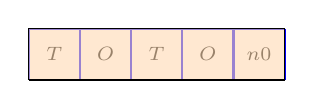
\begin{tikzpicture}[domain=0:5]
 \pgfmathsetmacro{\alpha}{0.05}
  \pgfmathsetmacro{\a}{0.65}
  %\draw[->] (0,0) -- (6*\a,0)  node[right] {$x$};
  %\draw[->] (0,0) -- (0,5.5*\a) node[left] {$y$};

  \foreach \n in {0,1,...,5}{
   \draw[blue,thick](\n*\a,0)-- ++(0,\a);
}
  \foreach \n in {0,1}{
    \draw[blue,thick](0,\n*\a)-- ++(5*\a,0);
}
\draw (0.5*\a,0.5*\a)  node {$\scriptstyle  T$};
\draw (1.5*\a,0.5*\a)  node {$\scriptstyle  O$};
\draw (2.5*\a,0.5*\a)  node {$\scriptstyle  T$};
\draw (3.5*\a,0.5*\a)  node {$\scriptstyle  O$};
\draw (4.5*\a,0.5*\a)  node {$\scriptstyle  \textbackslash0$};

\draw[fill=orange!30, fill opacity=0.6] (0,0)  -- ++(5*\a,0) -- ++(0,1*\a) -- ++(-5*\a,0) -- ++(0,-1*\a);

\end{tikzpicture}

\end{center}
Exemple : tableau 2 dimensions avec des chaines de caractères
\mint{c}|char Tab2D [5][7] ={"UN","DEUX","TROIS","QUATRE","CINQ"};|
On alloue le maximum pour ne pas avoir de problèmes de débordement.

 \begin{center}
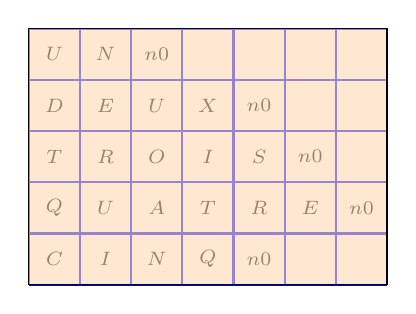
\begin{tikzpicture}[domain=0:5]
 \pgfmathsetmacro{\alpha}{0.05}
  \pgfmathsetmacro{\a}{0.65}
  %\draw[->] (0,0) -- (6*\a,0)  node[right] {$x$};
  %\draw[->] (0,0) -- (0,5.5*\a) node[left] {$y$};

  \foreach \n in {0,1,...,7}{
   \draw[blue,thick](\n*\a,0)-- ++(0,5*\a);
}
  \foreach \n in {0,1,...,5}{
    \draw[blue,thick](0,\n*\a)-- ++(7*\a,0);
}
\draw (0.5*\a,4.5*\a)  node {$\scriptstyle  U$};
\draw (1.5*\a,4.5*\a)  node {$\scriptstyle  N$};
\draw (2.5*\a,4.5*\a)  node {$\scriptstyle  \textbackslash0$};

\draw (0.5*\a,3.5*\a)  node {$\scriptstyle  D$};
\draw (1.5*\a,3.5*\a)  node {$\scriptstyle  E$};
\draw (2.5*\a,3.5*\a)  node {$\scriptstyle  U$};
\draw (3.5*\a,3.5*\a)  node {$\scriptstyle  X$};
\draw (4.5*\a,3.5*\a)  node {$\scriptstyle  \textbackslash0$};

\draw (0.5*\a,2.5*\a)  node {$\scriptstyle  T$};
\draw (1.5*\a,2.5*\a)  node {$\scriptstyle  R$};
\draw (2.5*\a,2.5*\a)  node {$\scriptstyle  O$};
\draw (3.5*\a,2.5*\a)  node {$\scriptstyle  I$};
\draw (4.5*\a,2.5*\a)  node {$\scriptstyle  S$};
\draw (5.5*\a,2.5*\a)  node {$\scriptstyle  \textbackslash0$};

\draw (0.5*\a,1.5*\a)  node {$\scriptstyle  Q$};
\draw (1.5*\a,1.5*\a)  node {$\scriptstyle  U$};
\draw (2.5*\a,1.5*\a)  node {$\scriptstyle  A$};
\draw (3.5*\a,1.5*\a)  node {$\scriptstyle  T$};
\draw (4.5*\a,1.5*\a)  node {$\scriptstyle  R$};
\draw (5.5*\a,1.5*\a)  node {$\scriptstyle  E$};
\draw (6.5*\a,1.5*\a)  node {$\scriptstyle  \textbackslash0$};

\draw (0.5*\a,0.5*\a)  node {$\scriptstyle  C$};
\draw (1.5*\a,0.5*\a)  node {$\scriptstyle  I$};
\draw (2.5*\a,0.5*\a)  node {$\scriptstyle  N$};
\draw (3.5*\a,0.5*\a)  node {$\scriptstyle  Q$};
\draw (4.5*\a,0.5*\a)  node {$\scriptstyle  \textbackslash0$};

\draw[fill=orange!30, fill opacity=0.6] (0,0)  -- ++(7*\a,0) -- ++(0,5*\a) -- ++(-7*\a,0) -- ++(0,-5*\a);

\end{tikzpicture}
\end{center}
Zone Mémoire inutilisables!!
\end{frame}

%%%%%%%%%%%%%%%%%%%%%%%%%%%%%%%%%%%%%%%%%%%%%%%%%%%%%%%%%%%%%%%%%
\begin{frame}[fragile]
\frametitle{Les tableaux en mémoire : Tableaux de pointeurs}
On déclare un tableau de pointeurs dans lequel chaque pointeur désigne l'adresse d'un autre tableau

Exemple : tableau 2 dimensions avec des chaines de caractères

\mint{c}|char *Tab2D [5] ;|

 \begin{center}
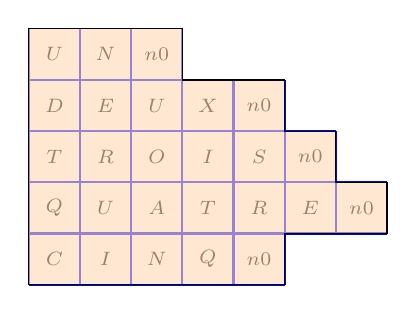
\begin{tikzpicture}[domain=0:5]
 \pgfmathsetmacro{\alpha}{0.05}
  \pgfmathsetmacro{\a}{0.65}
  %\draw[->] (0,0) -- (6*\a,0)  node[right] {$x$};
  %\draw[->] (0,0) -- (0,5.5*\a) node[left] {$y$};

\foreach \n in {0,1,...,3}{
   \draw[blue,thick](\n*\a,0)-- ++(0,5*\a);
}
\foreach \n in {4,5}{
   \draw[blue,thick](\n*\a,0)-- ++(0,4*\a);
}
\foreach \n in {6}{
   \draw[blue,thick](\n*\a,\a)-- ++(0,2*\a);
}
%%%%%%%%%%%%%%%%%%%%%%%%
\foreach \n in {0}{
    \draw[blue,thick](0,\n*\a)-- ++(5*\a,0);
}
\foreach \n in {1,2}{
    \draw[blue,thick](0,\n*\a)-- ++(7*\a,0);
}
\foreach \n in {3}{
    \draw[blue,thick](0,\n*\a)-- ++(6*\a,0);
}
\foreach \n in {4}{
    \draw[blue,thick](0,\n*\a)-- ++(5*\a,0);
}
\draw (0.5*\a,4.5*\a)  node {$\scriptstyle  U$};
\draw (1.5*\a,4.5*\a)  node {$\scriptstyle  N$};
\draw (2.5*\a,4.5*\a)  node {$\scriptstyle  \textbackslash0$};

\draw (0.5*\a,3.5*\a)  node {$\scriptstyle  D$};
\draw (1.5*\a,3.5*\a)  node {$\scriptstyle  E$};
\draw (2.5*\a,3.5*\a)  node {$\scriptstyle  U$};
\draw (3.5*\a,3.5*\a)  node {$\scriptstyle  X$};
\draw (4.5*\a,3.5*\a)  node {$\scriptstyle  \textbackslash0$};

\draw (0.5*\a,2.5*\a)  node {$\scriptstyle  T$};
\draw (1.5*\a,2.5*\a)  node {$\scriptstyle  R$};
\draw (2.5*\a,2.5*\a)  node {$\scriptstyle  O$};
\draw (3.5*\a,2.5*\a)  node {$\scriptstyle  I$};
\draw (4.5*\a,2.5*\a)  node {$\scriptstyle  S$};
\draw (5.5*\a,2.5*\a)  node {$\scriptstyle  \textbackslash0$};

\draw (0.5*\a,1.5*\a)  node {$\scriptstyle  Q$};
\draw (1.5*\a,1.5*\a)  node {$\scriptstyle  U$};
\draw (2.5*\a,1.5*\a)  node {$\scriptstyle  A$};
\draw (3.5*\a,1.5*\a)  node {$\scriptstyle  T$};
\draw (4.5*\a,1.5*\a)  node {$\scriptstyle  R$};
\draw (5.5*\a,1.5*\a)  node {$\scriptstyle  E$};
\draw (6.5*\a,1.5*\a)  node {$\scriptstyle  \textbackslash0$};

\draw (0.5*\a,0.5*\a)  node {$\scriptstyle  C$};
\draw (1.5*\a,0.5*\a)  node {$\scriptstyle  I$};
\draw (2.5*\a,0.5*\a)  node {$\scriptstyle  N$};
\draw (3.5*\a,0.5*\a)  node {$\scriptstyle  Q$};
\draw (4.5*\a,0.5*\a)  node {$\scriptstyle  \textbackslash0$};

\draw[fill=orange!30, fill opacity=0.6] (0,0)  -- ++(5*\a,0)-- ++(0,1*\a) -- ++(2*\a,0)  -- ++(0,\a) -- ++(-\a,0)-- ++(0,\a)-- ++(-\a,0)-- ++(0,\a) -- ++(-2*\a,0)-- ++(0,1*\a)-- ++(-3*\a,0)-- ++(0,-5*\a);

\end{tikzpicture}
\end{center}

\end{frame}
%%%%%%%%%%%%%%%%%%%%%%%%%%%%%%%%%%%%%%%%%%%%%%%%%%%%%%%%%%%%%%%%%

\begin{frame}[fragile]
\frametitle{Les tableaux en mémoire : Tableaux de pointeurs}
Exemple
\mint{c}|char Tab2D [5][7] ={"UN","DEUX","TROIS","QUATRE","CINQ"};|

\begin{minted}[
%frame=lines,
framesep=2mm,
baselinestretch=1.2,
bgcolor=LightGray,
fontsize=\footnotesize,
% linenos
]{c}
Tab[0]		//  pointe sur "UN"
Tab[1] 		//  pointe sur "DEUX"
*Tab[0]		//  retourne sur 'U' de "UN"
*( Tab[0] + 1) 	//  retourne sur 'N' de "UN"
*( Tab[1] + 2)	//  retourne sur 'U' de "DEUX"
\end{minted}
Attention l'expression:
\mint{c}|*Tab[4] + 1|	   
retourne 'D' car *Tab[4] => 'C' et 'C' + 1 => 'D'


\end{frame}

%%%%%%%%%%%%%%%%%%%%%%%%%%%%%%%%%%%%%%%%%%%%%%%%%%%%%%%%%%%%%%%%%

\begin{frame}[fragile]
\frametitle{Pointeur de pointeur:}
Un pointeur de pointeur est un pointeur pointant sur un pointeur, pointant sur un pointeur, . . . , pointant sur une variable. Cela permet de gérer des tableaux sans aucune dimension prédéfinie.
Exemple : tableau de chaine de caractère

\begin{minted}[
%frame=lines,
framesep=2mm,
baselinestretch=1.2,
bgcolor=LightGray,
fontsize=\footnotesize,
% linenos
]{c}
char *Tab[] = { "UN" , "DEUX", "TROIS", "QUATRE", "CINQ"} ;
char **p		// déclaration d'un pointeur de pointeur
p = &Tab[0]	// p pointe sur le début du tableau de chaines de caractères
		// * => chaine     ** => caractère
*p		//  pointe sur "UN" 
*(p+1) 		//  pointe sur "DEUX"
**p		//  retourne sur 'U' de "UN"
*(*p + 1) 	//  retourne sur 'N' de "UN"
*(*(p+1) + 2)	//  retourne sur 'U' de "DEUX"

\end{minted}

\end{frame}

%%%%%%%%%%%%%%%%%%%%%%%%%%%%%%%%%%%%%%%%%%%%%%%%%%%%%%%%%%%%%%%%%

\begin{frame}[fragile]
\frametitle{Allocation dynamique des pointeurs:}
La déclaration d'un pointeur n'engendre pas de réservation en mémoire. Si on ne réserve pas d'emplacement mémoire, le pointeur risque de pointer sur d'autres variables : débordement de pointeur. La réservation ou allocation mémoire pour les pointeurs est réalisée généralement dans une zone réservé appelé le tas (heap). On parle alors d'allocation dynamique (modifiable à tout moment par le programme).

On gère l'allocation dynamique de la mémoire avec les fonctions suivantes:
\begin{itemize}
\item {\tt malloc()}
\item {\tt calloc()}
\item {\tt realloc()}
\item {\tt free()}
\end{itemize}

\end{frame}

%%%%%%%%%%%%%%%%%%%%%%%%%%%%%%%%%%%%%%%%%%%%%%%%%%%%%%%%%%%%%%%%%

\begin{frame}[fragile]
\frametitle{Allocation dynamique des pointeurs:}
La fonction {\tt malloc()} : 
\mint{c}|void *malloc(taille);|
\begin{itemize}
\item Elle alloue un bloc de mémoire de {\tt taille} octets sur le tas
\item Elle renvoie un pointeur sur la zone de type {\tt void} (valable pour tous les types) qu'il faut donc convertir en un type adapté aux données.
\item Si l'allocation réussit, {\tt malloc} renvoi un pointeur sur le bloc, elle échoue si {\tt taille = 0} ou s'il n'y a pas assez de place en mémoire. Dans ce cas elle retourne un pointeur nul : {\tt NULL}
\end{itemize}
\begin{minted}[
%frame=lines,
framesep=2mm,
baselinestretch=1.2,
bgcolor=LightGray,
fontsize=\footnotesize,
% linenos
]{c}
int *p;
p = (int *) malloc(10 * sizeof(int) ); // réservation pour 10 entiers
if ( p== NULL){   // test création du pointeur	
	printf("erreur d'allocation mémoire !!!");
	// ici traitement de l'erreur …
} 
\end{minted}
\end{frame}

%%%%%%%%%%%%%%%%%%%%%%%%%%%%%%%%%%%%%%%%%%%%%%%%%%%%%%%%%%%%%%%%%

\begin{frame}[fragile]
\frametitle{Allocation dynamique des pointeurs:}
\begin{minted}[
%frame=lines,
framesep=2mm,
baselinestretch=1.2,
bgcolor=LightGray,
fontsize=\footnotesize,
% linenos
]{c}
#include <stdio.h>
#include <stdlib.h>

int main () {
    int n=0,i=0,*t= NULL;
    printf("Veuillez entrer la taille du tableau : ");
    scanf("%d",&n);
    t=malloc(sizeof(int)*n);
    for(i=0;i<n;++i){
        printf("Veuillez entrer un nombre : ");
        scanf("%d", &t[i]);
    }
    for(i=0;i<n;++i){
        printf("Nombre %d : %d\n",(i+1),t[i]);
    }
    free(t);
    return 0;
}

\end{minted}
\end{frame}

%%%%%%%%%%%%%%%%%%%%%%%%%%%%%%%%%%%%%%%%%%%%%%%%%%%%%%%%%%%%%%%%%

\begin{frame}[fragile]
\frametitle{Allocation dynamique des pointeurs:}
La fonction {\tt calloc()} : 
\mint{c}|void *calloc(nombre,taille);|
\begin{itemize}
\item Elle alloue un bloc de mémoire de {\tt nombre x taille} octets sur le tas
\item Elle renvoie un pointeur sur la zone de type {\tt void} (valable pour tous les types) qu'il faut donc convertir en un type adapté aux données.
\item Si l'allocation réussit, {\tt calloc} renvoi un pointeur sur le bloc, elle échoue si {\tt taille = 0} ou s'il n'y a pas assez de place en mémoire. Dans ce cas elle retourne un pointeur nul : {\tt NULL}
\end{itemize}
\begin{minted}[
%frame=lines,
framesep=2mm,
baselinestretch=1.2,
bgcolor=LightGray,
fontsize=\footnotesize,
% linenos
]{c}
int *p;
p = (int *) calloc(10 , sizeof(int) ); // réservation pour 10 entiers
if ( p== NULL){   // test création du pointeur	
	printf("erreur d'allocation mémoire !!!");
	// ici traitement de l'erreur …
} 
\end{minted}
\end{frame}

%%%%%%%%%%%%%%%%%%%%%%%%%%%%%%%%%%%%%%%%%%%%%%%%%%%%%%%%%%%%%%%%%

\begin{frame}[fragile]
\frametitle{Allocation dynamique des pointeurs:}
\begin{minted}[
%frame=lines,
framesep=2mm,
baselinestretch=1.2,
bgcolor=LightGray,
fontsize=\footnotesize,
% linenos
]{c}
#include <stdio.h>
#include <stdlib.h>

int main () {
    int n=0,i=0,*t= NULL;
    printf("Veuillez entrer la taille du tableau : ");
    scanf("%d",&n);
    t=calloc(n, sizeof(int));
    for(i=0;i<n;++i){
        printf("Veuillez entrer un nombre : ");
        scanf("%d", &t[i]);
    }
    for(i=0;i<n;++i){
        printf("Nombre %d : %d\n",(i+1),t[i]);
    }
    free(t);
    return 0;
}

\end{minted}
\end{frame}
%%%%%%%%%%%%%%%%%%%%%%%%%%%%%%%%%%%%%%%%%%%%%%%%%%%%%%%%%%%%%%%%%

\begin{frame}[fragile]
\frametitle{Allocation dynamique des pointeurs:}
La fonction {\tt realloc()} : 
\mint{c}|void *realloc(pointeur,newtaille);|
\begin{itemize}
\item Elle permet de changer la taille d'un bloc déjà alloué. Elle gère l'aspect dynamique des pointeurs. Utilisable à tous moment dans le programme
\item Elle renvoie un pointeur sur la zone de type {\tt void} (valable pour tous les types) qu'il faut convertir en un type adapté aux données.
\item Si l'allocation réussit, {\tt realloc} renvoi un pointeur sur le bloc, elle échoue si {\tt taille = 0} ou s'il n'y a pas assez de place en mémoire. Dans ce cas elle retourne un pointeur nul : {\tt NULL}
\end{itemize}
\begin{minted}[
%frame=lines,
framesep=2mm,
baselinestretch=1.2,
bgcolor=LightGray,
fontsize=\footnotesize,
% linenos
]{c}
int *p;
...
p = (int *) realloc(p , 20*sizeof(int) ); // réservation pour 10 entiers supplémentaires
if ( p== NULL){   // test création du pointeur	
	printf("erreur d'allocation mémoire !!!");
	// ici traitement de l'erreur …
} //ATTENTION, les données peuvent être déplacées si l'espace n'est pas suffisant !!!
\end{minted}
\end{frame}

%%%%%%%%%%%%%%%%%%%%%%%%%%%%%%%%%%%%%%%%%%%%%%%%%%%%%%%%%%%%%%%%%

\begin{frame}[fragile]
\frametitle{Allocation dynamique des pointeurs:}
\begin{minted}[
%frame=lines,
framesep=2mm,
baselinestretch=1.2,
bgcolor=LightGray,
fontsize=\footnotesize,
% linenos
]{c}
#include <stdio.h>
#include <stdlib.h>
int main () {
    int n=0,i=0;
    int *t= NULL;
    printf("Veuillez entrer la taille du tableau : ");
    scanf("%d",&n);
    t=malloc(n * sizeof(int));
    for(i=0;i<n;++i){
        printf("Veuillez entrer un nombre : ");
        scanf("%d", &t[i]);
    }
    t=realloc(t,sizeof(int)*(n+1));
    t[n]=100;
    for(i=0;i<=n;++i) printf("Nombre %d : %d\n",i+1,t[i]);
    free(t);
    return 0;
}
\end{minted}
\end{frame}
%%%%%%%%%%%%%%%%%%%%%%%%%%%%%%%%%%%%%%%%%%%%%%%%%%%%%%%%%%%%%%%%%

\begin{frame}[fragile]
\frametitle{Allocation dynamique des pointeurs:}
La fonction {\tt free()} : 
\mint{c}|free ( pointeur );|
\begin{itemize}
\item Elle permet de libérer l'espace mémoire alloué par les fonctions {\tt malloc(), calloc() realloc()}
\item Il est très important de libérer l'espace mémoire après utilisation, sinon celui-ci devient inutilisable pour la suite du programme
\end{itemize}
\begin{minted}[
%frame=lines,
framesep=2mm,
baselinestretch=1.2,
bgcolor=LightGray,
fontsize=\footnotesize,
% linenos
]{c}
int *p;
p = (int *) malloc(10*sizeof(int) ); // réservation pour 10 entiers
if ( p== NULL){   // test création du pointeur	
	printf("erreur d'allocation mémoire !!!");
	// ici traitement de l'erreur …
} 
...
...
free(p);// on libère la mémoire
\end{minted}
\end{frame}

%%%%%%%%%%%%%%%%%%%%%%%%%%%%%%%%%%%%%%%%%%%%%%%%%%%%%%%%%%%%%%%%%

\begin{frame}[fragile]
\frametitle{Allocation dynamique des pointeurs:}
\begin{minted}[
%frame=lines,
framesep=2mm,
baselinestretch=1.2,
bgcolor=LightGray,
fontsize=\footnotesize,
% linenos
]{c}
#include <stdio.h>
#include <stdlib.h>
int main () {
    int n=0,i=0;
    int *t= NULL;
    printf("Veuillez entrer la taille du tableau : ");
    scanf("%d",&n);
    t=malloc(n * sizeof(int));
    if (t==NULL) return -1;
    for(i=0;i<n;++i){
        printf("Veuillez entrer un nombre : ");
        scanf("%d", &t[i]);
    }
    for(i=0;i<n;++i)  printf("Nombre %d : %d\n",i+1,t[i]);
    free(t);
    return 0;
}
\end{minted}
\end{frame}

%%%%%%%%%%%%%%%%%%%%%%%%%%%%%%%%%%%%%%%%%%%%%%%%%%%%%%%%%%%%%%%%%

\begin{frame}[fragile]
\frametitle{tableaux sur la pile}
\begin{enumerate}
\item taille importante = stack overflow 
\item durée de vie associée à la fonction !
\end{enumerate}
\begin{minted}[
%frame=lines,
framesep=2mm,
baselinestretch=1.2,
bgcolor=LightGray,
fontsize=\footnotesize,
% linenos
]{c}
#include <stdio.h>
#include <stdlib.h>
int * function (int n){
    int tab[n];
    for(int i=0;i<n;i++) tab[i]=i;
    return tab ;
}
int main(){
    int* tab, n=3;
    tab = function (n) ;
    for(int i=0;i<n;i++)
        printf("%d\n",tab[i]) ;
    free(tab);
    return 0;
}
\end{minted}
\end{frame}

%%%%%%%%%%%%%%%%%%%%%%%%%%%%%%%%%%%%%%%%%%%%%%%%%%%%%%%%%%%%%%%%%

\begin{frame}[fragile]
\frametitle{tableaux sur la pile}
\begin{enumerate}
\item solution : allocation dynamique (voir prochain cours)
\end{enumerate}
\begin{minted}[
%frame=lines,
framesep=2mm,
baselinestretch=1.2,
bgcolor=LightGray,
fontsize=\footnotesize,
% linenos
]{c}
#include <stdio.h>
#include <stdlib.h>
int * function (int n){
    int* tab = (int*) malloc(n*sizeof(int));
    for(int i=0;i<n;i++) tab[i]=i;
    return tab ;
}
int main(){
    int* tab, n=3;
    tab = function (n) ;
    for(int i=0;i<n;i++)
        printf("%d\n",tab[i]) ;
    free(tab);
    return 0;
}
\end{minted}
\end{frame}

\end{document}
